\chapter{Results}
\label{cha:chapter4}

In this chapter, we present the results of the analysis carried out on the road network of the city of Mérida. We start with a characterization of the complete network, at municipal scale, on Section~\ref{sec:municipal-scale}. Then, we scale down, and characterize the network of each individual AGEB, where in Section~\ref{sec:ageb-scale} we present aggregated results. Finally, we show clustering results on the AGEBs in Section~\ref{sec:clustering}, that display signs of spatial correlation within the city.

\section{Municipal scale}
\label{sec:municipal-scale}

Table~\ref{tab:measures_urban_city} presents statistics for the Mérida's municipality street network.

Mérida has 35031 intersections and 5 million meters of linear street.
It is 96\% less circuitous than straight-line edges would be. The average street segment length (a proxy for block size) is 99 meters. It has 31 intersections per km$^2$.

\begin{table*}[htbp]
  \centering
  \caption{Selected measures of all Mérida street network.}
  \label{tab:measures_urban_city}
  \small
  \begin{tabular}{ l r }
    \toprule
    measure                                          &              \\
    \midrule
    Area (km\textsuperscript{2})                     & 1032.365    \\
    Avg of the avg neighborhood degree               & 2.843        \\
    Avg of the avg weighted neighborhood degree      & 0.045       \\
    Avg circuity                                     & 0.964 \\
    Avg clustering coefficient                       & 0.030        \\
    Avg weighted clustering coefficient              & 0.001 \\
    Intersection count                               & 31837      \\
    Avg degree centrality                            & \textless0.001          \\
    Edge density (km/km\textsuperscript{2})          & 9013.845         \\
    Avg edge length (m)                              & 99.662          \\
    Total edge length (km)                           & 9306      \\
    Proportion of dead-ends                          & 0.091          \\
    Proportion of 3-way intersections                & 0.592         \\
    Proportion of 4-way intersections                & 0.312          \\
    Intersection density (per km\textsuperscript{2}) & 30.839          \\
    $m$                                              & 93371     \\
    $n$                                              & 35031      \\
    Node density (per km\textsuperscript{2})         & 33.933         \\
    Max PageRank value                               & \textless0.001 \\
    Min PageRank value                               & \textless0.001 \\
    Self-loop proportion                             & 0.001        \\
    Street density (km/km\textsuperscript{2})        & 5259.333        \\
    Average street segment length (m)                & 99.177        \\
    Total street length (km)                         & 5430     \\
    Street segment count                             & 54746      \\
    Average streets per node                         & 3.130         \\
    \bottomrule
  \end{tabular}
\end{table*}

The distribution of node types (i.e., intersections and dead ends) provides an indicator of network connectedness.
Mérida has 3.1 streets per intersection on average; 31\% of nodes are 4-way intersections, 59\% are 3-way intersections, and 9\% are dead-ends (see Figure \ref{fig:merida-node-types-distribution}).

\begin{figure}[htpb]
  \centering
  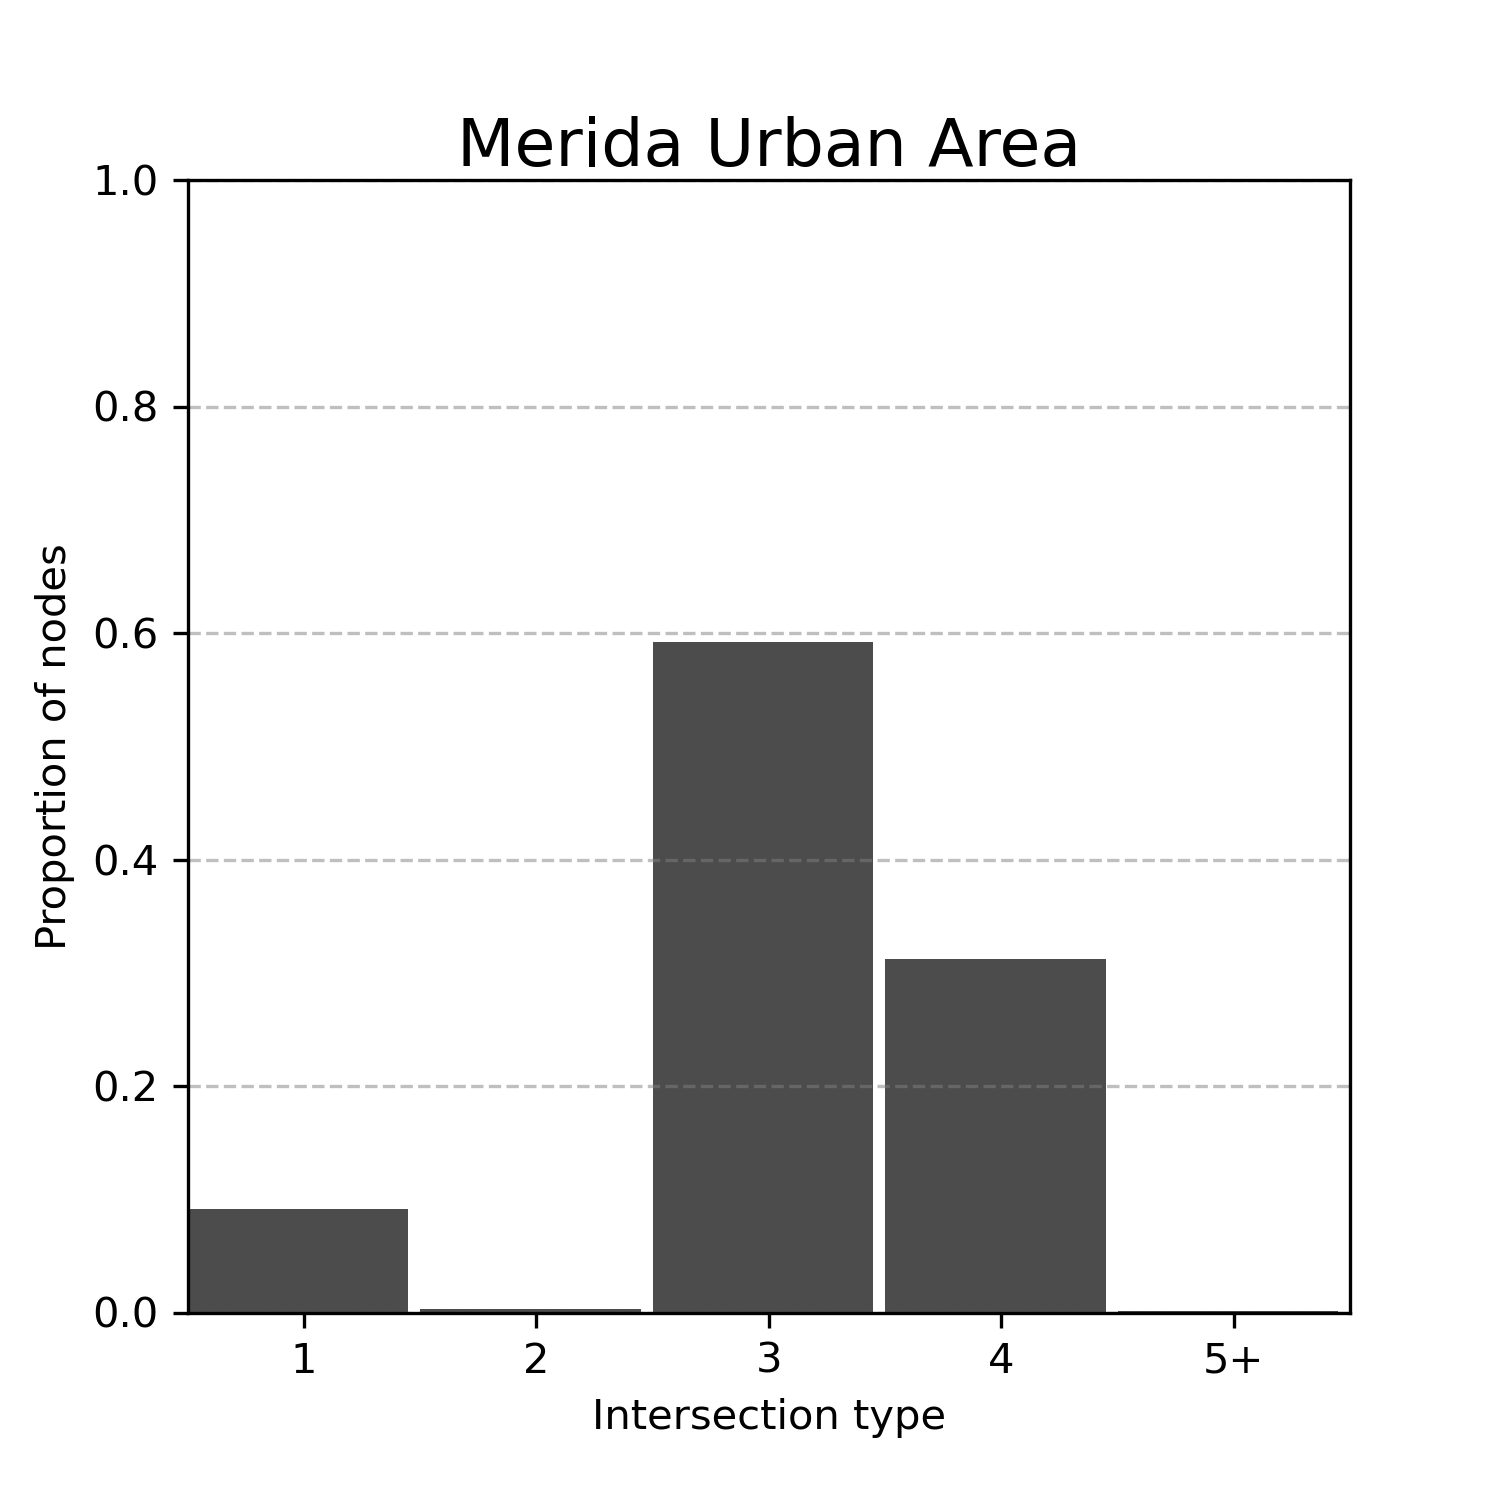
\includegraphics[width=0.5\textwidth]{Figures/merida-street-per-node-proportion-distribution.png}
  \caption{Distribution of node types in Mérida. It has 3.1 streets per intersection on average; 31\% of nodes are 4-way intersections, 59\% are 3-way intersections, and 9\% are dead-ends.
    \label{fig:merida-node-types-distribution}}
\end{figure}

Centrality measures identify the most important nodes in a network.
We can have different ways of thinking about importance.
Some of the most known centrality measures are: degree centrality, closeness centrality, betweenness centrality, and PageRank.
Each of these measures gives us a different approach, or use case, to identify the most important nodes in the network~\cite{menczer_fortunato_davis_2020}.

According to degree centrality, important nodes have many connections.
Figure~\ref{fig:merida-max-node-degree-centrality} depicts the node with highest degree centrality.
This node is at the intersection of many streets that pass through it.
In Figure~\ref{fig:merida-degree-centrality} we can visualize all nodes by their relative degree centrality.
We can observe that intersections in principal streets, avenues, and in the historical center of Mérida have low degree centrality compared to intersections in residential areas.

\begin{figure}[htpb]
  \centering
  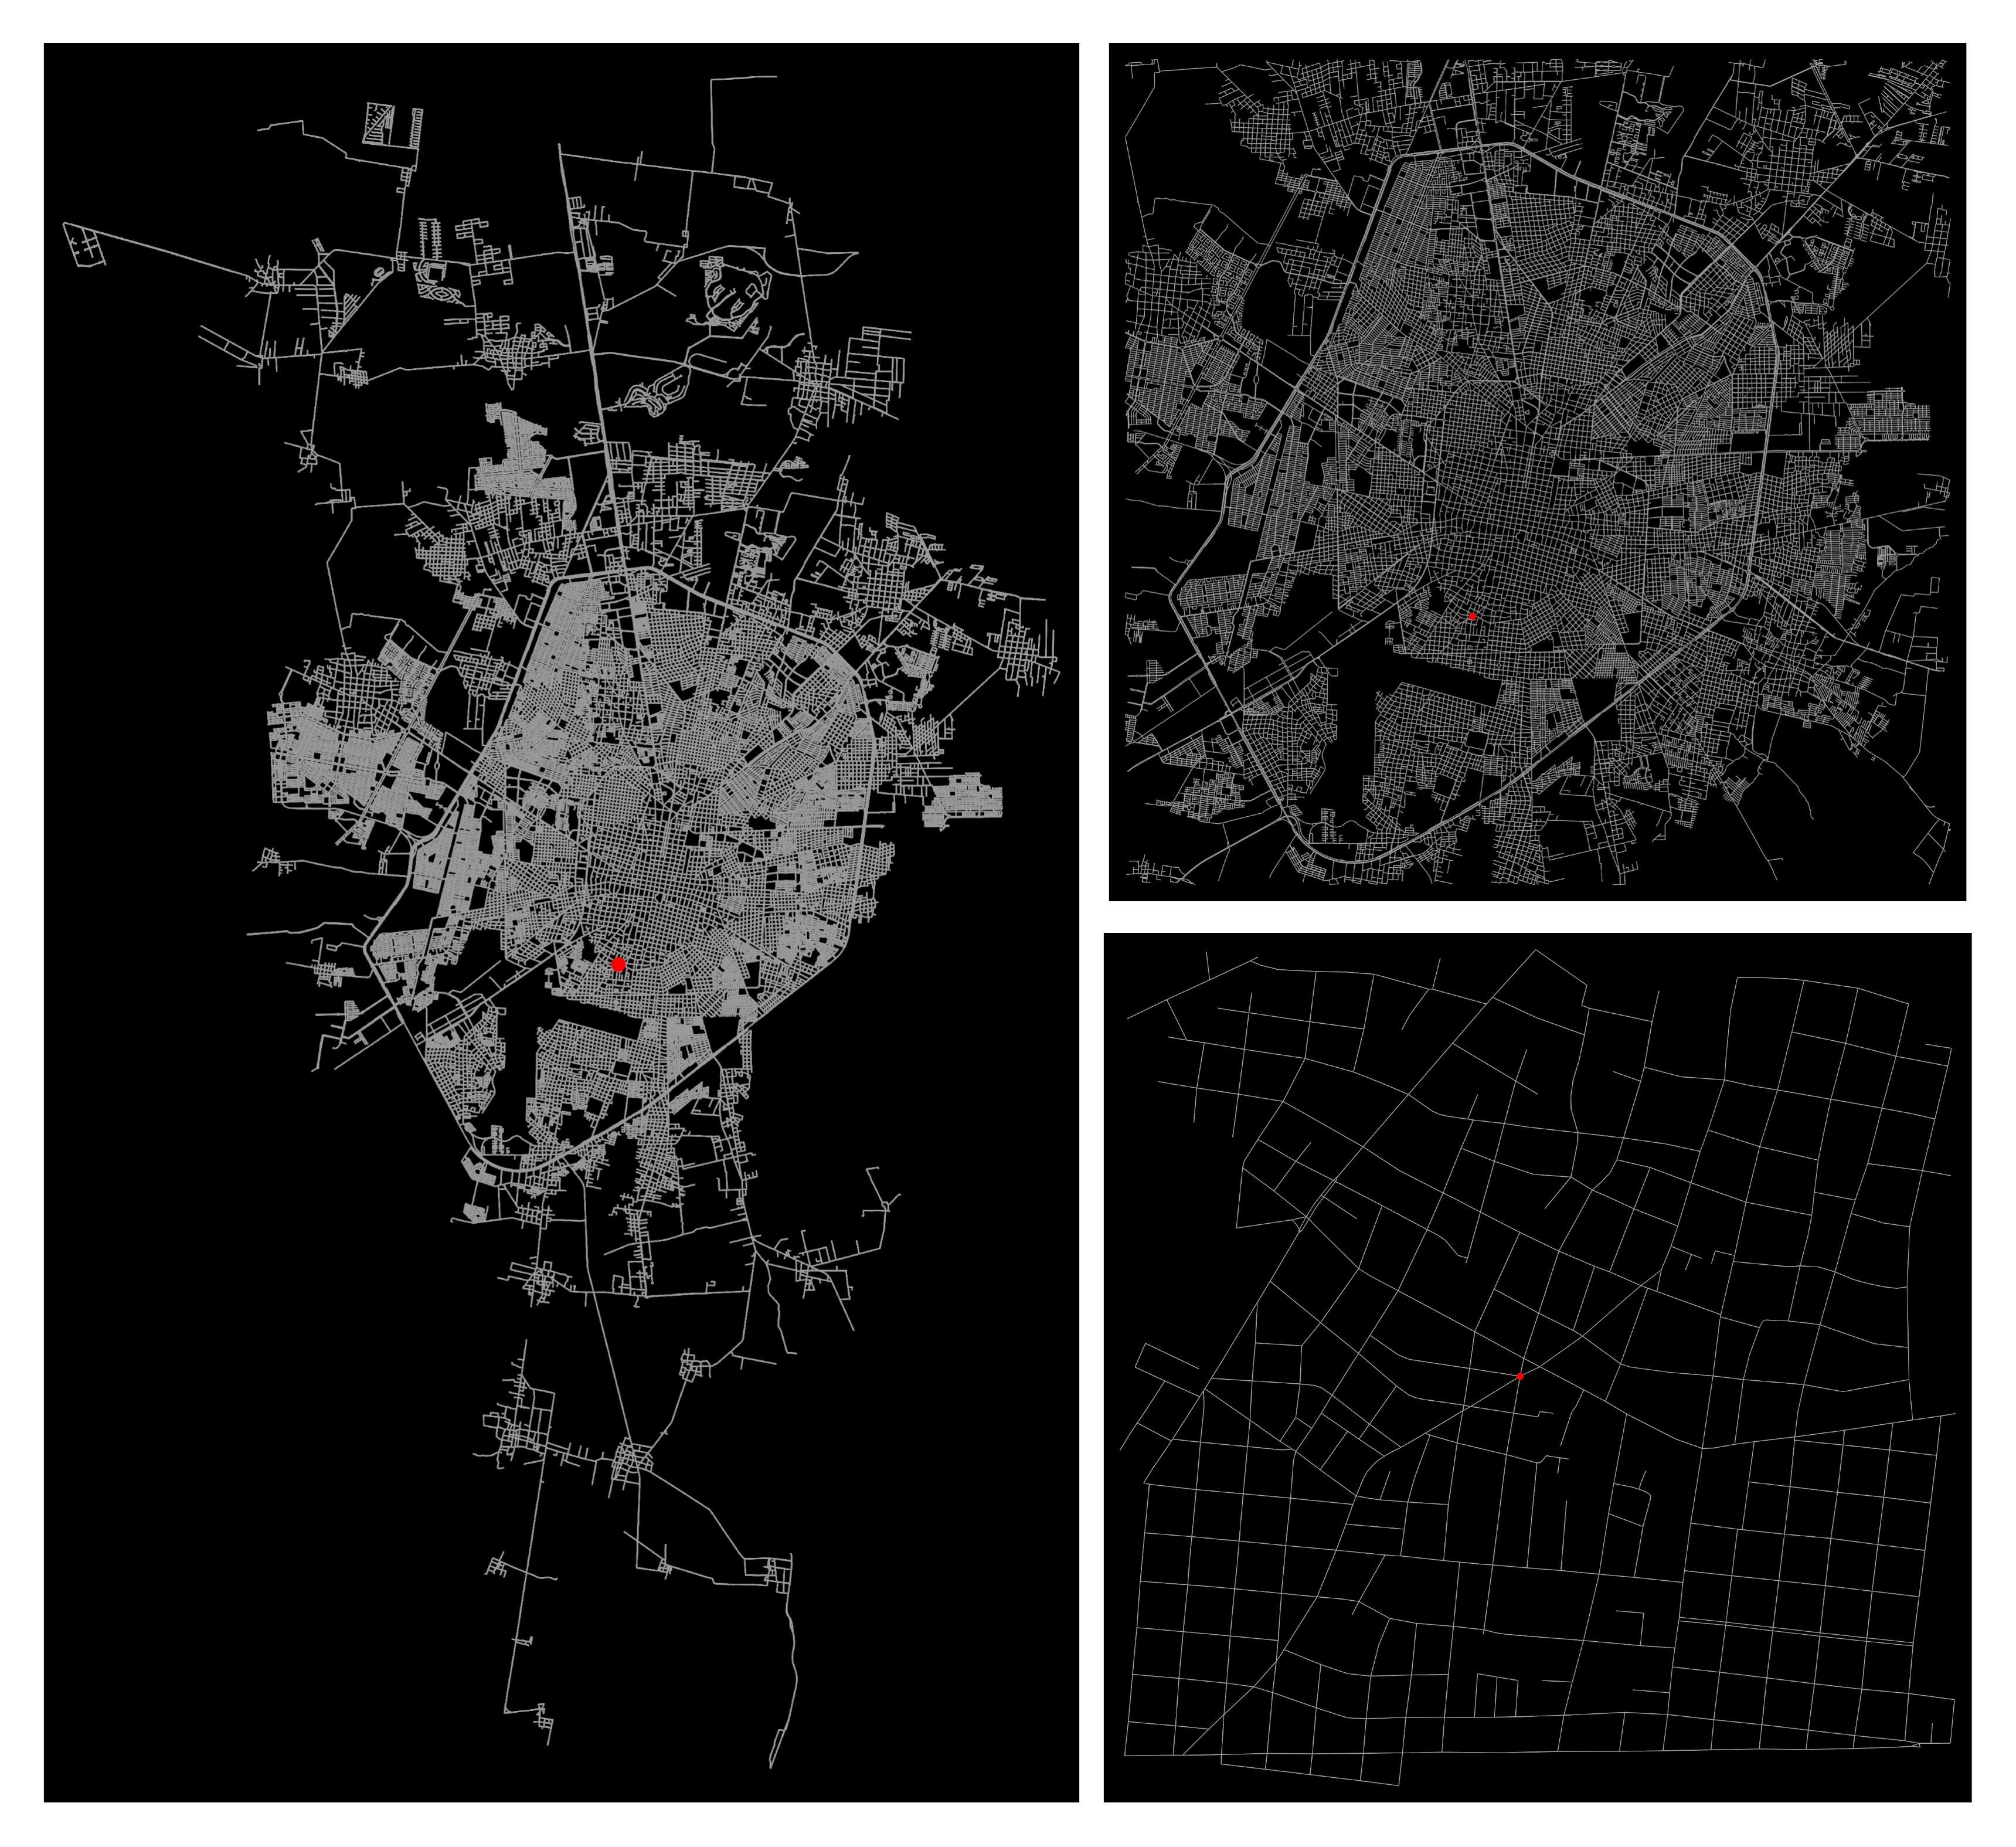
\includegraphics[width=1.0\textwidth]{Figures/merida-node-degree-centrality.png}
  \caption{Node with highest degree centrality score. The node is located at 64 street with 95 and 75 street, colonia Meliton Salazar.
    \label{fig:merida-max-node-degree-centrality}}
\end{figure}

\begin{figure}[htpb]
  \centering
  \includegraphics[width=0.8\textwidth]{Figures/merida-degree-centrality.png}
  \caption{Degree centrality of all nodes in Mérida. Nodes are visualized from low (dark violet) to high (light yellow). The colors in colorspace are linearly mapped to the attribute values. observe that intersections in principal streets, avenues, and in the historical center of Mérida have low degree centrality compared to intersections in residential areas.
    \label{fig:merida-degree-centrality}}
\end{figure}

Closeness centrality makes the assumption that important nodes are close to other nodes. Figure \ref{fig:merida-max-node-closeness-centrality} depicts the node with highest closeness centrality. This node is closer to all other nodes in the network, which makes sense because it is an important intersection in Mérida. In Figure \ref{fig:merida-closeness-centrality} we can observe how nodes in the south and outside Mérida city are less important according to closeness centrality, while nodes at the historical center, north, and even north-west are more important. We also calculate closeness centrality for edges (street roads) (see Figure \ref{fig:merida-edge-closeness-centrality}) and we observe that the peripheral ring road from west to north is the most important road as well as those roads closer to it. Additionally, we can observe the great difference of importance from the south peripheral ring road to all the other segments of the peripheral ring road of Mérida city.

\begin{figure}[htpb]
  \centering
  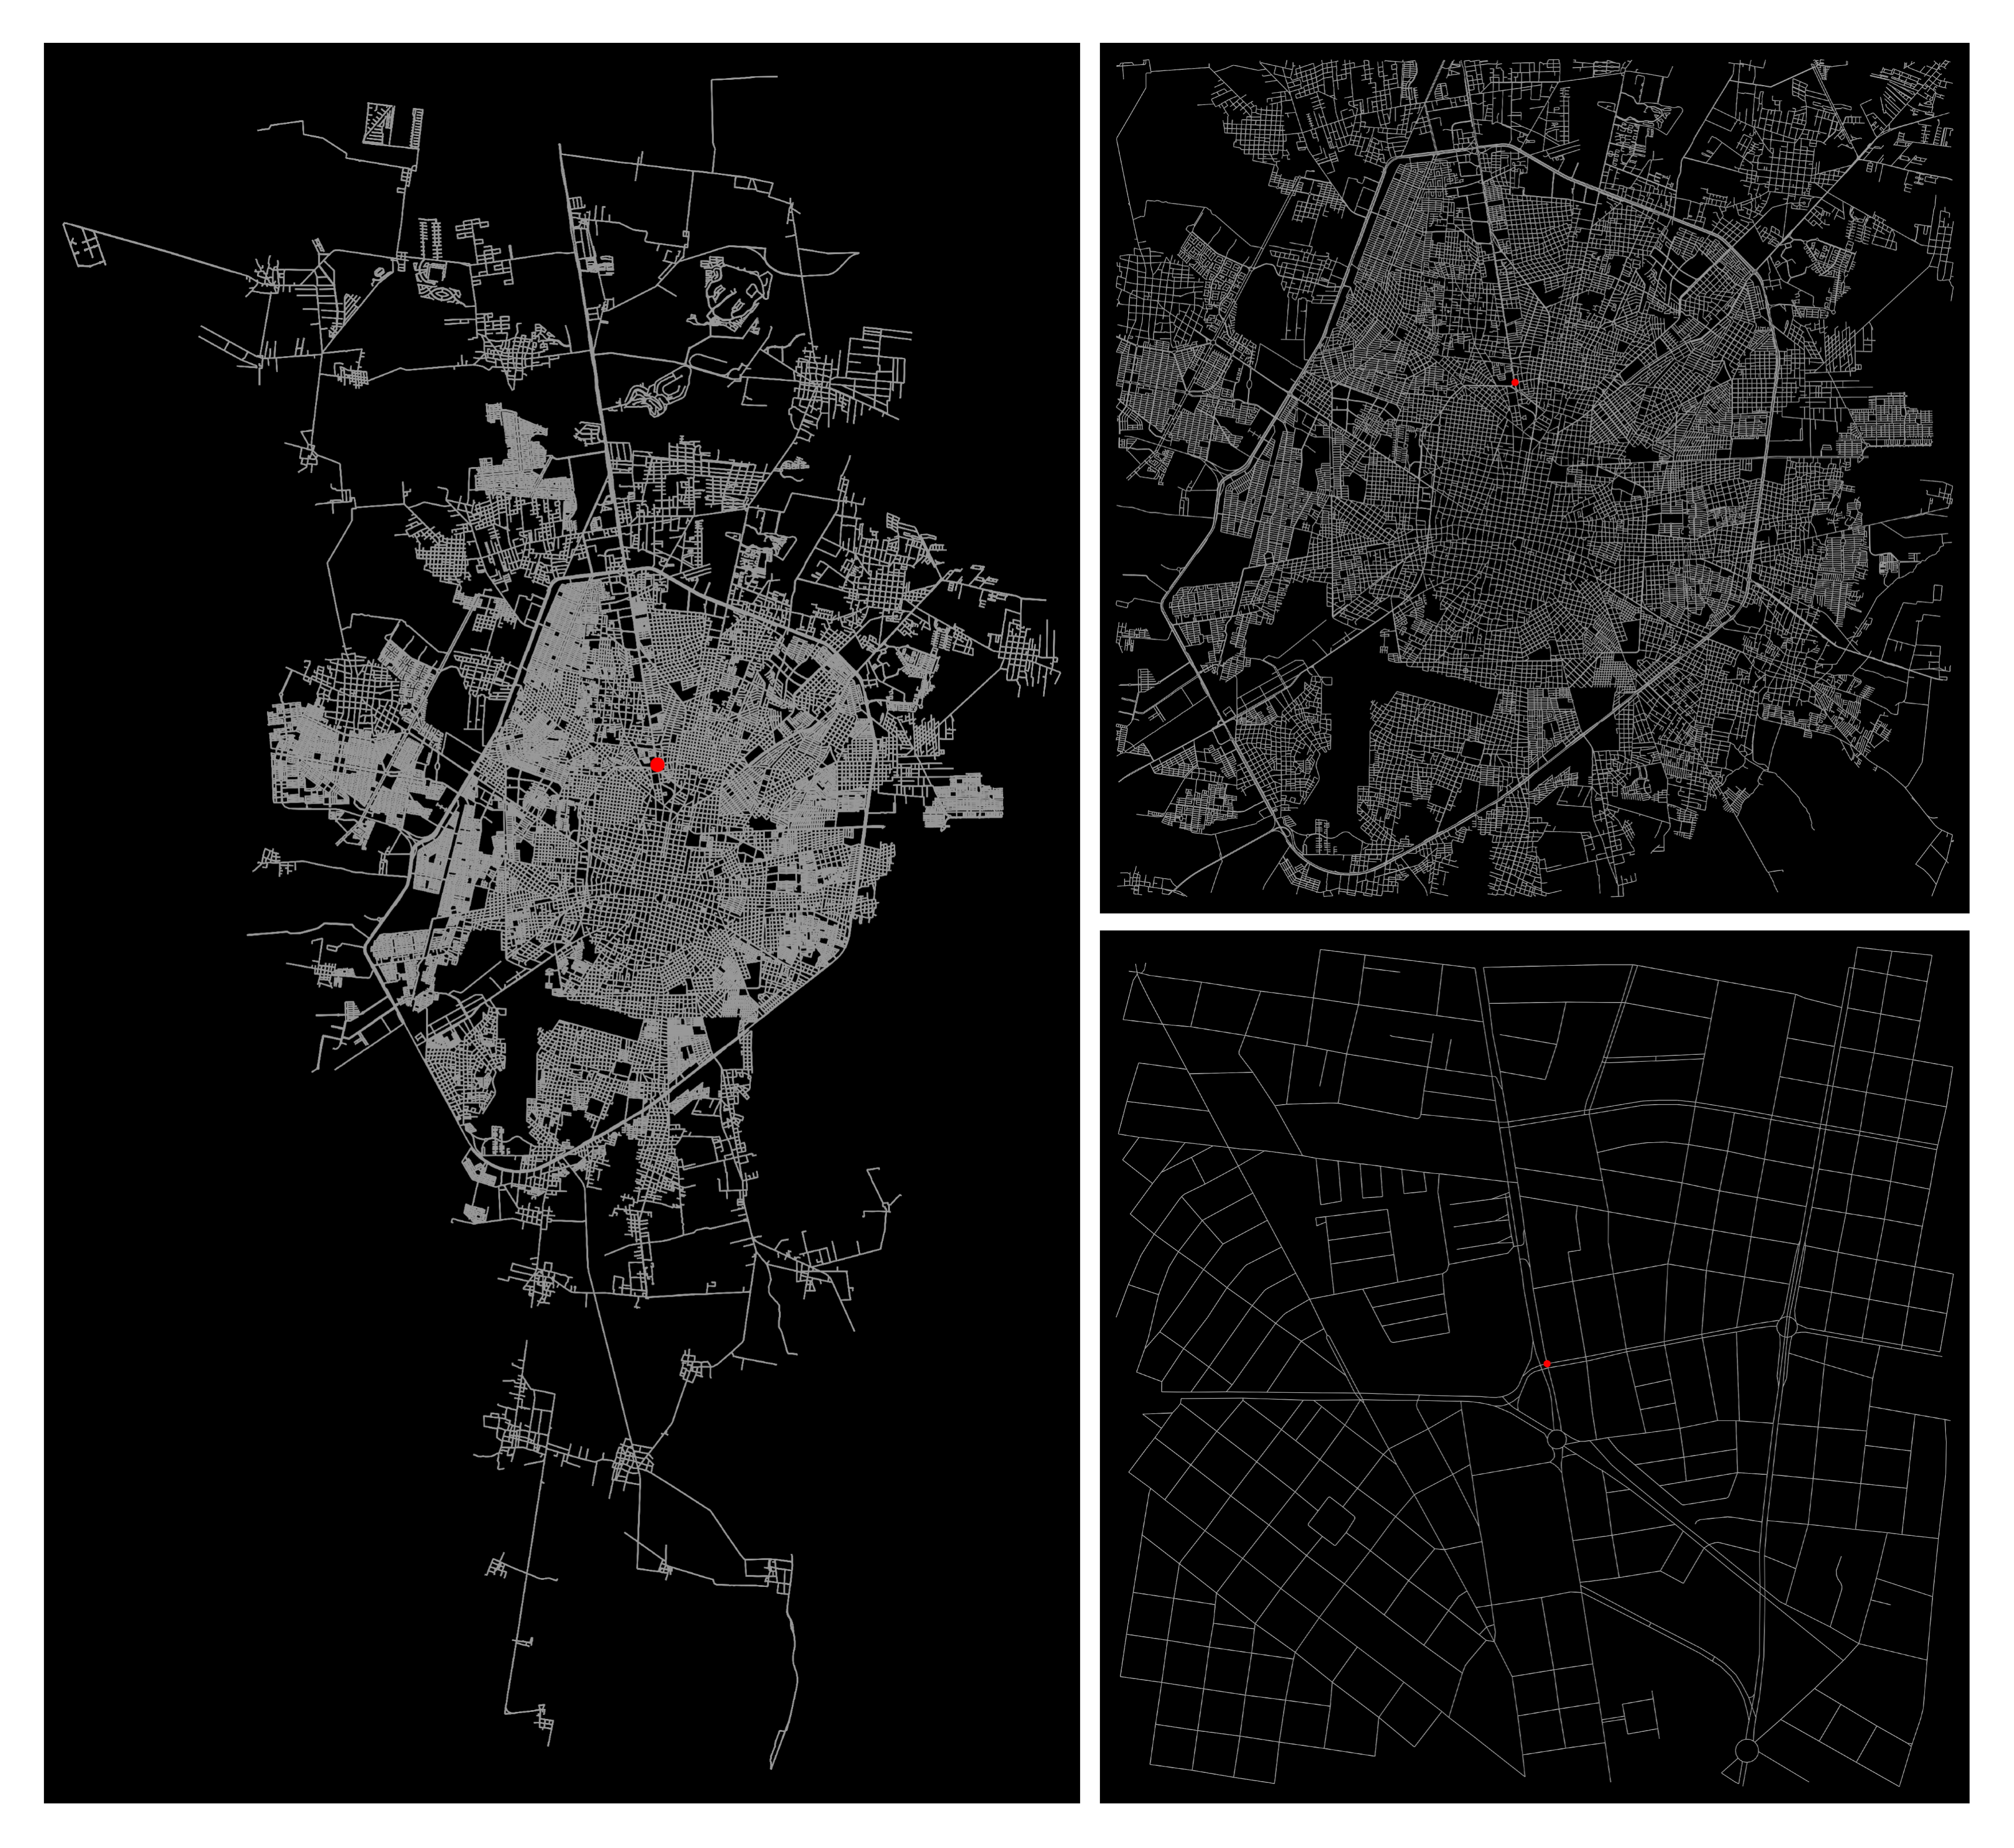
\includegraphics[width=1.0\textwidth]{Figures/merida-node-closeness-centrality.png}
  \caption{Node with highest closeness centrality score. This node is located at the Circuito Colonias and 60 street.
    \label{fig:merida-max-node-closeness-centrality}}
\end{figure}

\begin{figure}[htpb]
  \centering
  \includegraphics[width=0.8\textwidth]{Figures/merida-closeness-centrality.png}
  \caption{Closeness centrality of all nodes in Mérida. Nodes are visualized from low (dark violet) to high (light yellow). Observe how nodes in the south and outside Mérida city are less important according to closeness centrality, while nodes at the historical center, north, and even north-west are more important.
    \label{fig:merida-closeness-centrality}}
\end{figure}

\begin{figure}[htpb]
  \centering
  \includegraphics[width=0.8\textwidth]{Figures/merida-edge-closeness-centrality.png}
  \caption{Closeness centrality of all edges in Mérida. Edges are visualized from low (dark) to high (light yellow). Observe that the peripheral ring road from west to north is the most important road as well as those roads closer to it. Additionally, we can observe the great difference of importance from the south peripheral ring road to all the other segments of the peripheral ring road of Mérida city.
    \label{fig:merida-edge-closeness-centrality}}
\end{figure}

Betweenness centrality declares that important nodes are those who connect other nodes; it is also a measure to examine resilience in the network. In Mérida, the node highlighted in red has approximately 7\% of all shortest paths running through it (see Figure \ref{fig:merida-max-node-betweenness-centrality}). If we observe Figure \ref{fig:merida-betweenness-centrality}, see that intersections in principal avenues and streets are the most important, which makes sense because they connect the city in a more efficient way.

\begin{figure}[htpb]
  \centering
  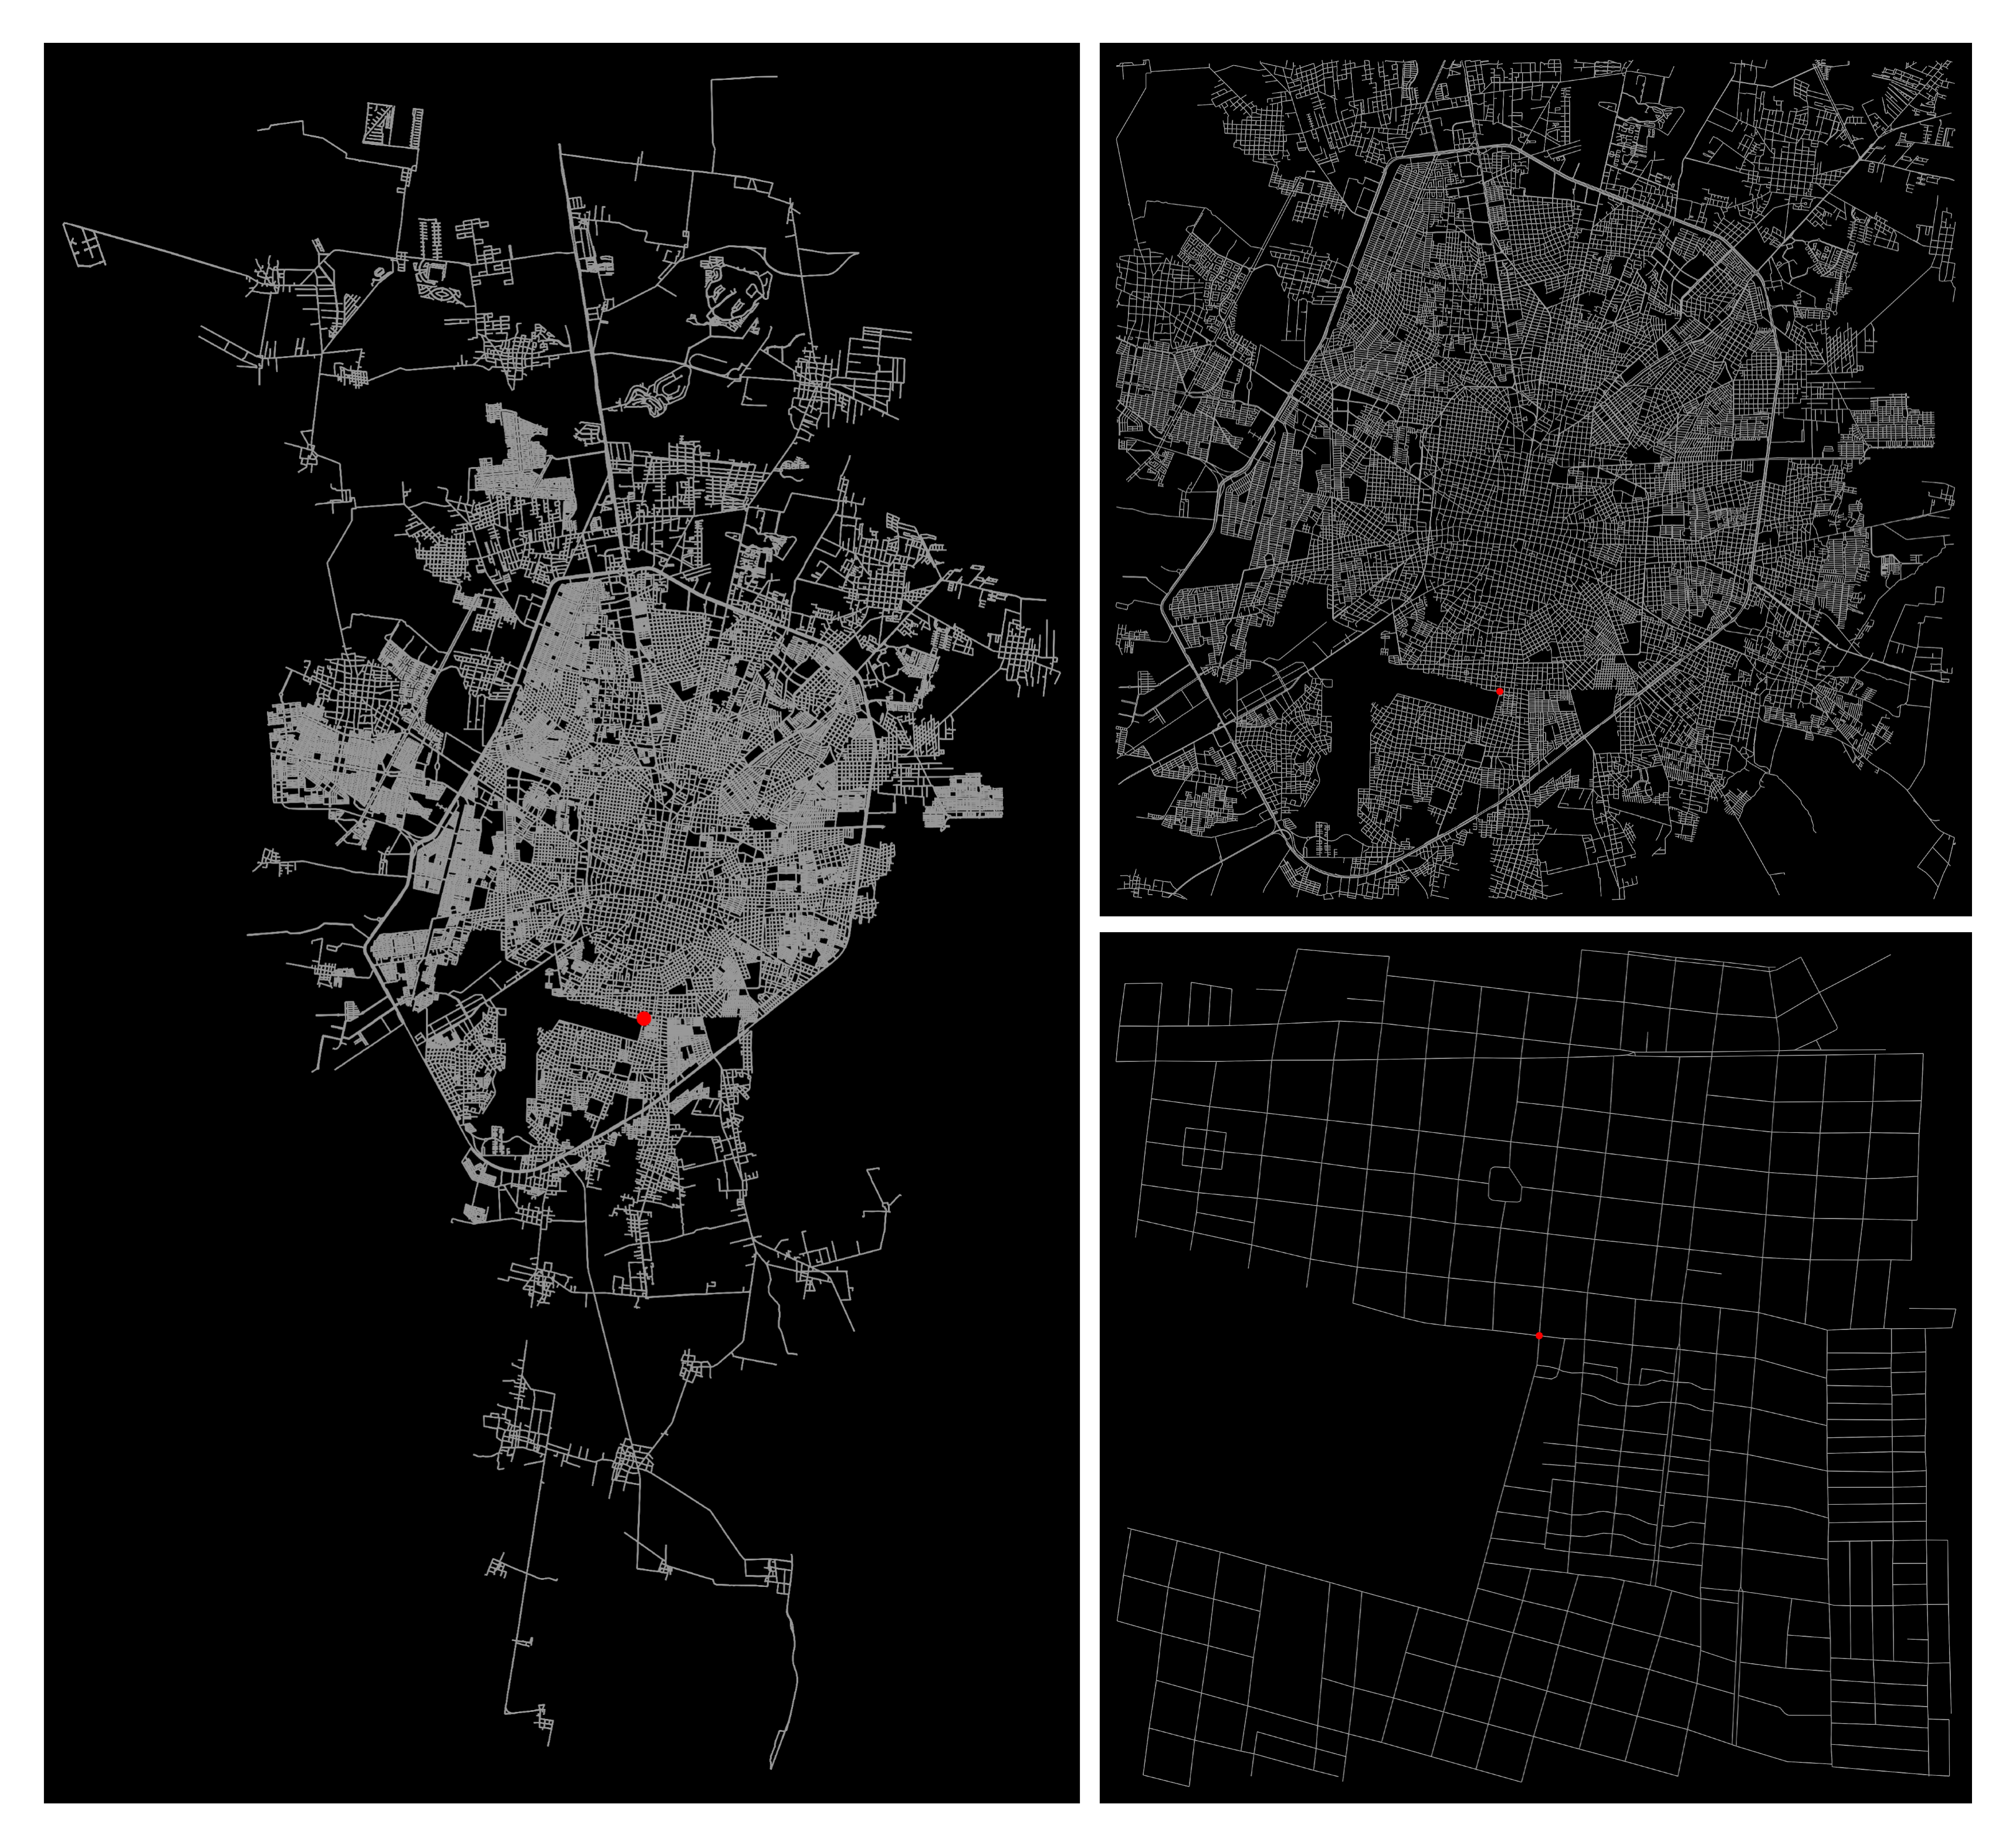
\includegraphics[width=1.0\textwidth]{Figures/merida-node-betweenness-centrality.png}
  \caption{Node with highest betweenness centrality score. This node is the intersection at 121 street and 54 street, colonia Mercedes Barrera.
    \label{fig:merida-max-node-betweenness-centrality}}
\end{figure}

\begin{figure}[htpb]
  \centering
  \includegraphics[width=0.8\textwidth]{Figures/merida-betweenness-centrality.png}
  \caption{Betweenness centrality of all nodes in Mérida. Nodes are visualized from low (dark violet) to high (light yellow). See that intersections in principal avenues and streets are the most important because they connect the city in a more efficient way.
    \label{fig:merida-betweenness-centrality}}
\end{figure}

Finally, PageRank makes the assumption that important nodes are those that have many in-links from other important nodes; this measure is useful for directed networks. The node with highest PageRank is presented in Figure \ref{fig:merida-max-node-pagerank}. This node is important because it is connected to other important nodes, which makes sense because it is located at one of the most important avenues in Mérida city.

\begin{figure}[htpb]
  \centering
  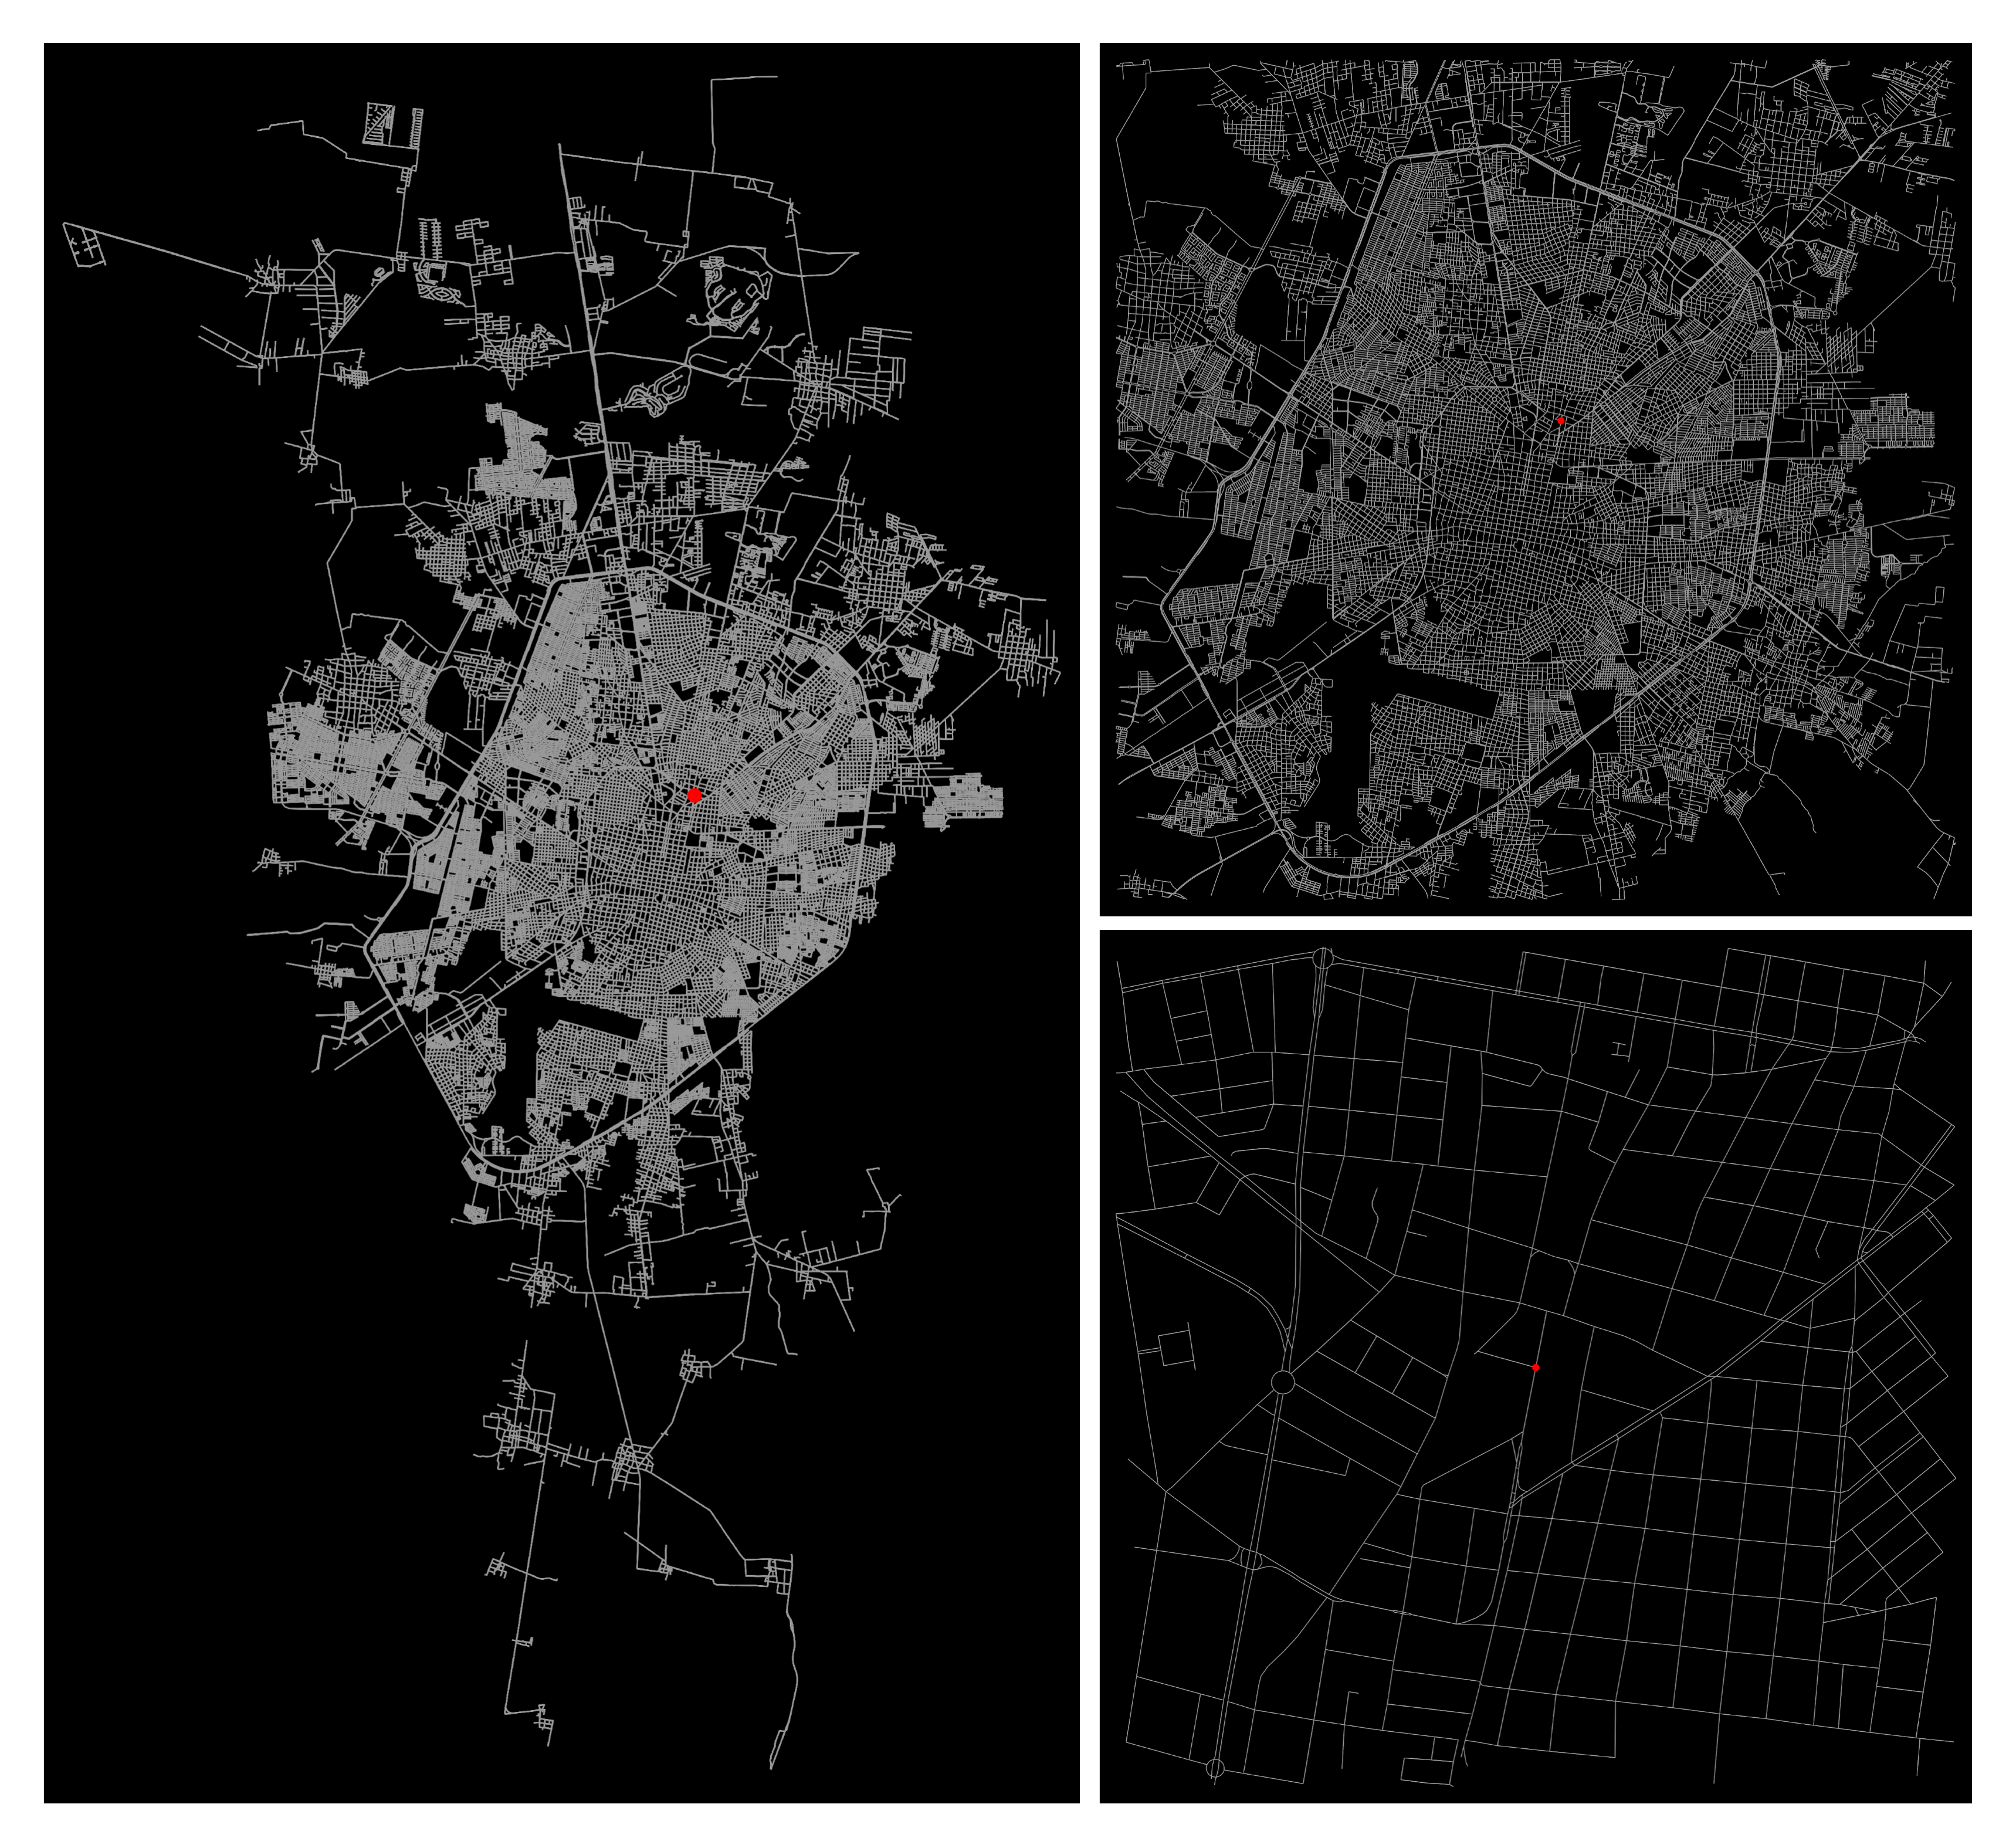
\includegraphics[width=1.0\textwidth]{Figures/merida-node-pagerank.png}
  \caption{Node with highest PageRank score. This node is located at Rotary Internacional Av. and 21A street, colonia Itzimna. This node is important because it is connected to other important nodes, which makes sense because it is located at one of the most important avenues in Mérida city.
    \label{fig:merida-max-node-pagerank}}
\end{figure}

\section{AGEB scale}
\label{sec:ageb-scale}

While the municipal scale captures planning decisions made by the city government, the neighborhood, or, in this case, AGEB represent the scale of individual urban design intervertions into the urban form \cite{boeing_multi-scale_2018}. Additionally, this scale reflects the street network development in different eras, designs, and paradigms individually.

Table \ref{tab:measures_urban_agebs} presents summary statistics for the 513 AGEBs analyzed in this work. The typical AGEB has 3.2 streets per intersection (see Figure \ref{fig:merida-ageb-histograms}a), reflecting the prevalence of 3-way intersections in the municipality, discussed earlier. The median proportions of each node type are 3.1\% for dead-ends, 58.5\% for 3-way intersections, and 34.9\% for 4-way intersections. The typical AGEB averages 92-meter street segment lengths (Figure \ref{fig:merida-ageb-histograms}b) and 112.8 intersections per km$^2$ (Figure \ref{fig:merida-ageb-histograms}c).

\begin{figure}[htpb]
  \centering
  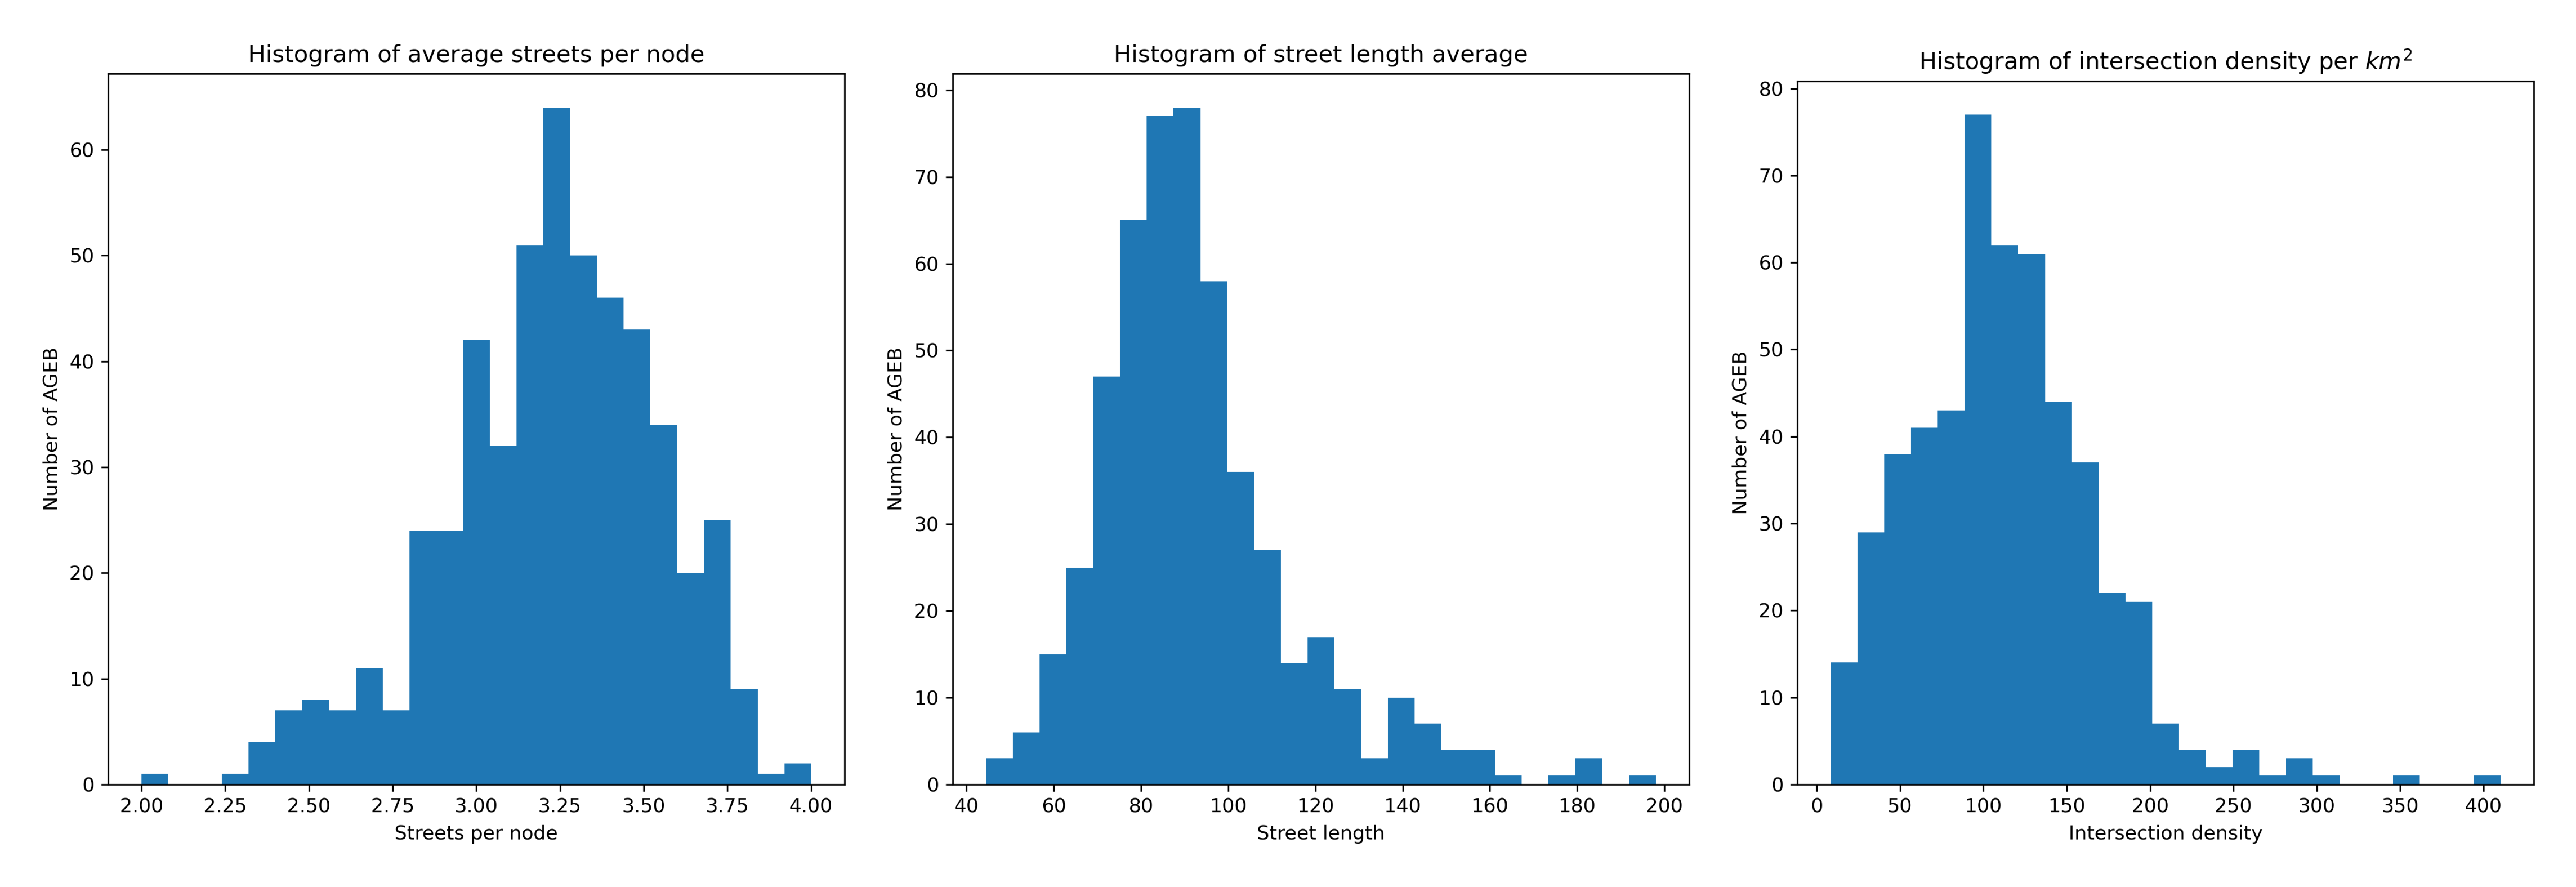
\includegraphics[width=\textwidth]{Figures/merida-ageb-histograms.png}
  \caption{Histograms of average streets per node (left) shows that the typical AGEB has 3.2 streets per intersection; the typical AGEB averages 92-meter street segment lengths (middle), and has 112.8 intersections per km$^2$ (right).
    \label{fig:merida-ageb-histograms}}
\end{figure}

In Figure \ref{fig:merida-ageb-street-length-vs-nodes} , we examine the relationship between the total street length and the number of nodes across the AGEBs, and we find a meaningful linear relationship ($r^2 = 0.81$). The not-so-strong linear relationship is due to the fact that we are handling invariant street networks designed and shaped in different historical eras.

\begin{figure}[htpb]
  \centering
  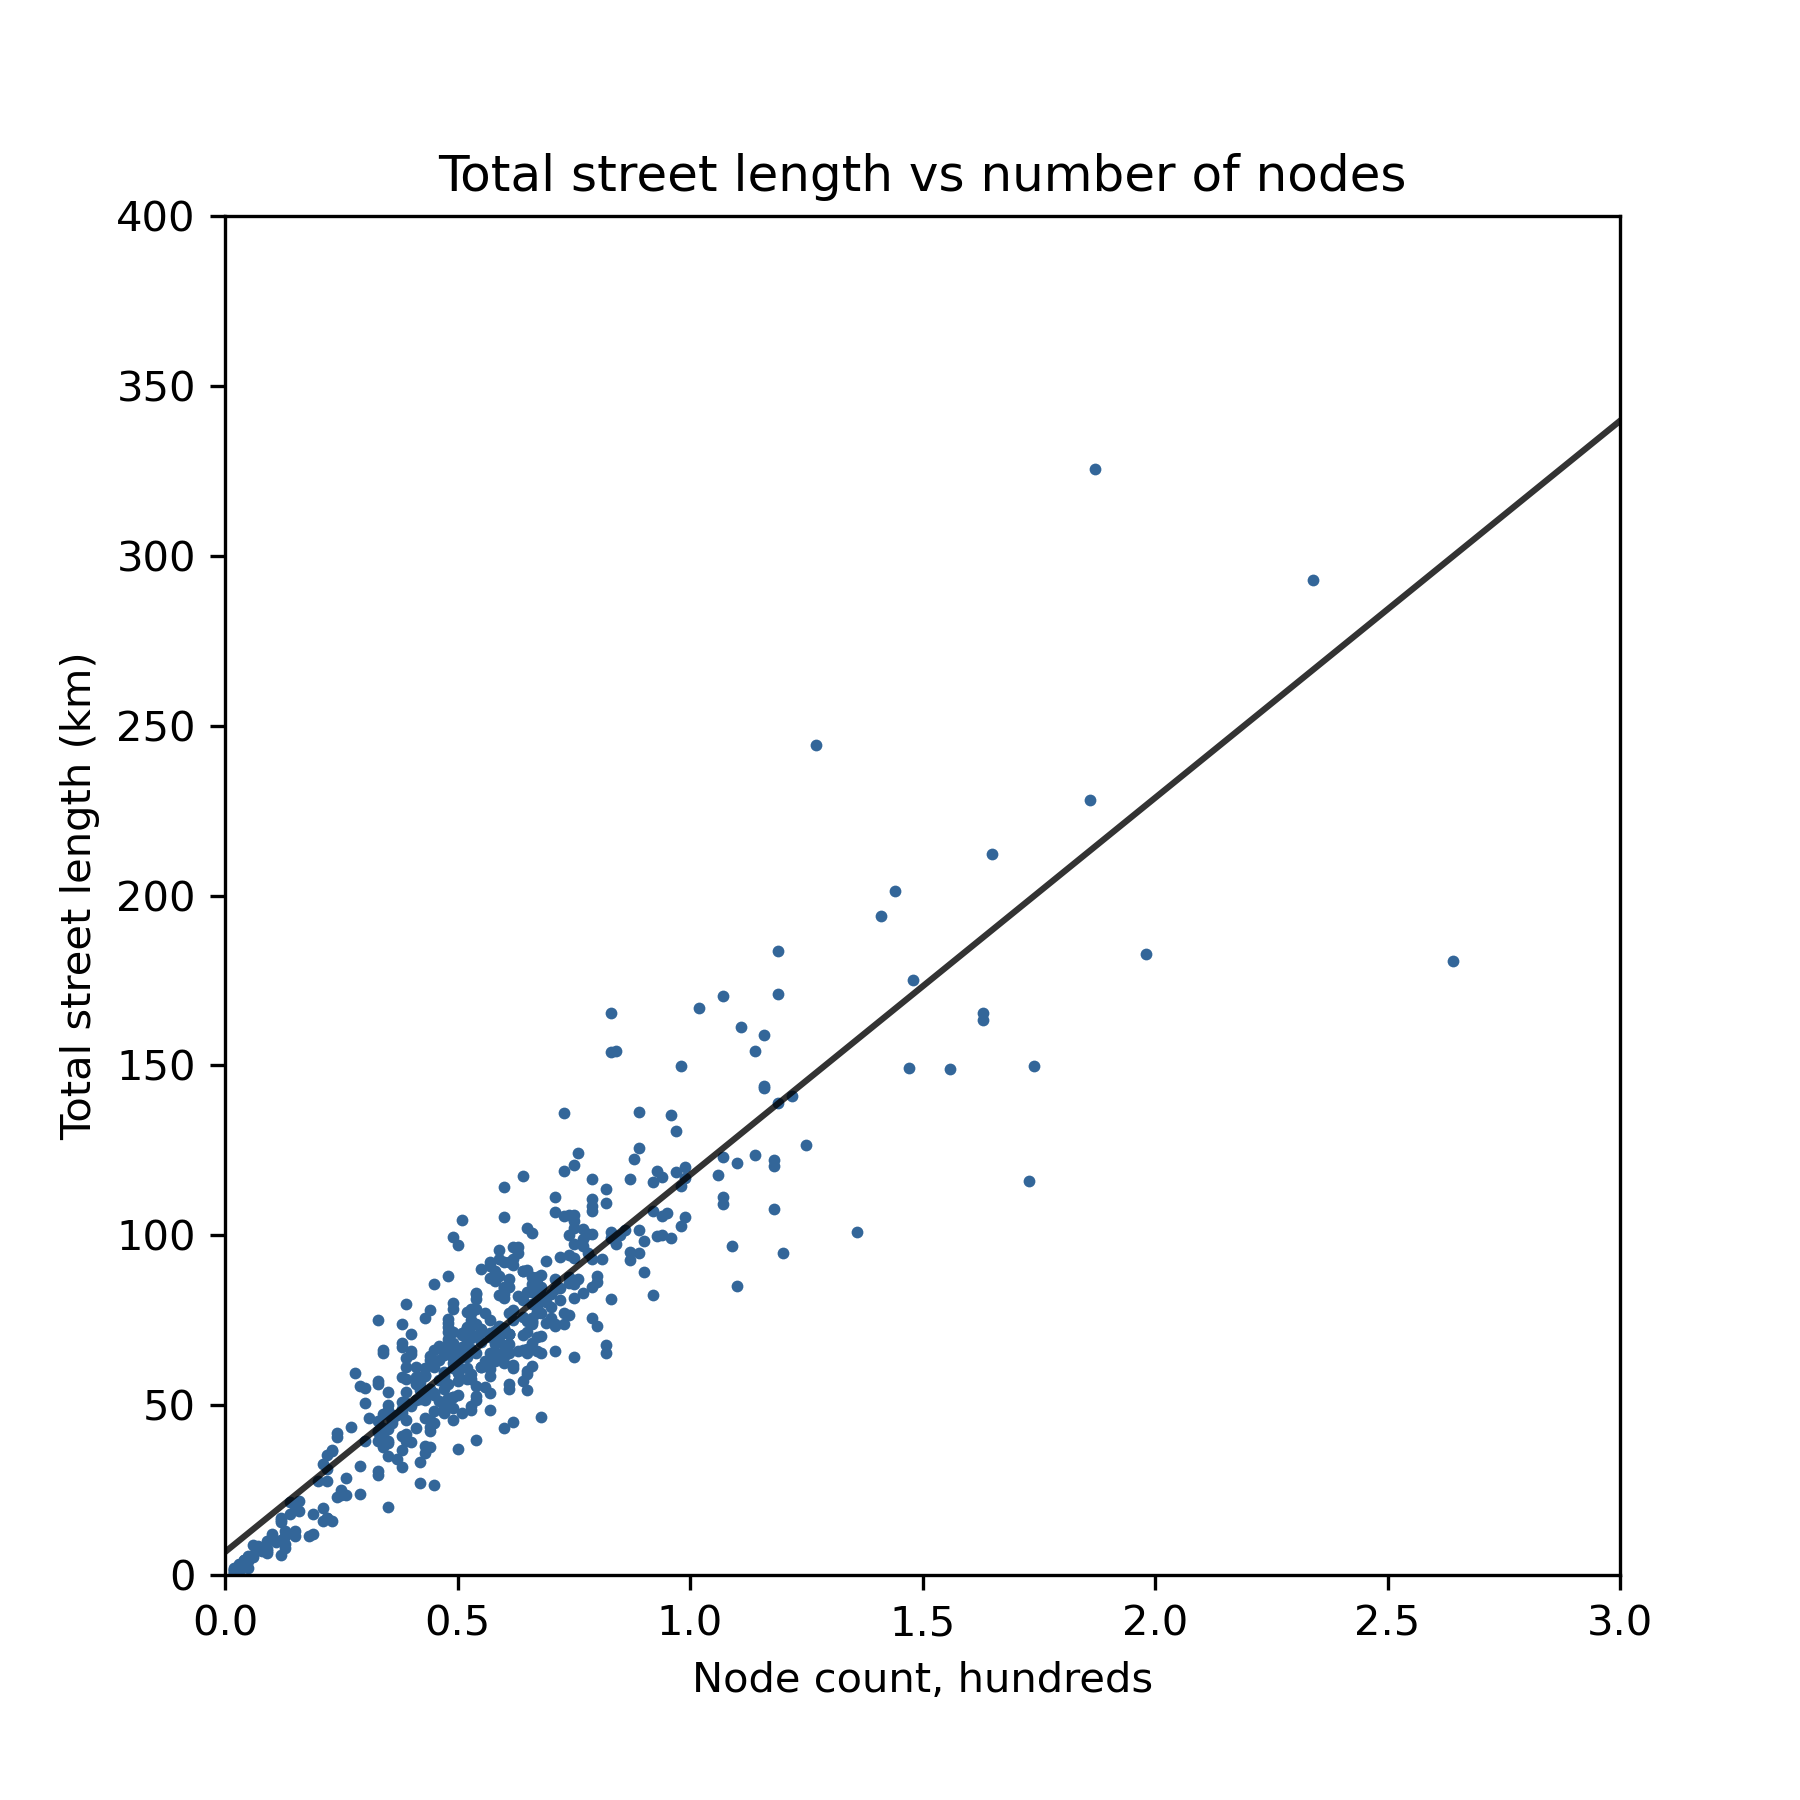
\includegraphics[width=0.5\textwidth]{Figures/merida-ageb-street-length-vs-nodes.png}
  \caption{Linear relationship between total street length and number of nodes in the street network of every Mérida urban AGEB. We find a meaningful linear relationship ($r^2 = 0.81$). The not-so-strong linear relationship is due to the fact that we are handling invariant street networks designed and shaped in different historical eras.
    \label{fig:merida-ageb-street-length-vs-nodes}}
\end{figure}

\begin{landscape}
\begin{table*}[htbp]
  \centering
  \caption{Central tendency and statistical dispersion for selected measures of all Mérida urban AGEB's street networks: $\mu$ is the mean, $\sigma$ is the standard deviation, and $D$ is the dispersion index $\frac{\sigma ^ 2}{\mu}$.}
  \label{tab:measures_urban_agebs}
  \small
  \begin{tabular}{ l r r r r r r }
    \toprule
    measure                                          & $\mu$          & $\sigma$       & min            & median         & max            & $D$            \\
    \midrule
    Area (km\textsuperscript{2})                     & 0.582        & 0.527        & 0.014         & 0.475        & 7.613       & 0.477       \\
    Avg of the avg neighborhood degree               & 2.477          & 0.470          & 0.500          & 2.556          & 3.414          & 0.089          \\
    Avg of the avg weighted neighborhood degree      & 0.039          & 0.012          & 0.005          & 0.039          & 0.097          & 0.004          \\
    Avg circuity                                     & 0.960          & 0.066          & 0.932          & 0.940          & 1.741          & 0.005 \\
    Avg clustering coefficient                       & 0.027          & 0.044          & 0          & 0.017          & 0.583          & 0.072          \\
    Avg weighted clustering coefficient              & 0.007          & 0.02          & 0 & 0.003          & 0.397          & 0.057 \\
    Intersection count                               & 53.393          & 29.065          & 1            & 52           & 204         & 15.664      \\
    Avg degree centrality                            & 0.156          & 0.270          & 0.015 & 0.088          & 2          & 0.467          \\
    Edge density (km/km\textsuperscript{2})          & 23657.180         & 8967.089          & 1543.392          & 23866.890         & 47341.220         & 3398.913          \\
    Avg edge length (m)                              & 92.625        & 23.339         & 44.488        & 88.761        & 237.350        & 5.881          \\
    Total edge length (km)                           & 12.153           & 7.015          & 0.01            & 11.47           & 49.218         & 4.05      \\
    Proportion of dead-ends                          & 0.069          & 0.089          & 0          & 0.031          & 0.500          & 0.115          \\
    Proportion of 3-way intersections                & 0.566          & 0.179          & 0          & 0.585          & 1          & 0.057          \\
    Proportion of 4-way intersections                & 0.373          & 0.190          & 0.006          & 0.349          & 1          & 0.097          \\
    Intersection density (per km\textsuperscript{2}) & 112.849         & 54.826          & 8.403         & 108.692         & 410.011         & 26.636          \\
    Average node degree                              & 1.348          & 0.488          & 0.163          & 1.333          & 2.772          & 0.177          \\
    $m$                                              & 136.035          & 11.534          & 2           & 130          & 528         & 44.191     \\
    $n$                                              & 58.193          & 33.431          & 2            & 54           & 264         & 19.206      \\
    Node density (per km\textsuperscript{2})         & 120.451         & 57.043          & 9.226         & 116.253         & 410.011         & 27.014          \\
    Max PageRank value                               & 0.063          & 0.082          & 0.001 & 0.039          & 0.500          & 0.107 \\
    Min PageRank value                               & 0.016 & 0.060 & 0.001 & 0.003 & 0.500 & 0.225 \\
    Self-loop proportion                             & 0.001          & 0.004          & 0 & 0          & 0.046          & 0.016         \\
    Street density (km/km\textsuperscript{2})        & 13743.660          & 4999.535          & 774.708          & 13920.640          & 28345.930         & 1818.683          \\
    Average street segment length (m)                & 92.472        & 22.521         & 44.488        & 88.585        & 198.010        & 5.485          \\
    Total street length (km)                         & 7.134           & 4.120           & 0.045            & 6.750           & 32.542          & 2.375      \\
    Street segment count                             & 79.803          & 45.775          & 1           & 76           & 321         & 26.257      \\
    Average streets per node                         & 3.225          & 0.320          & 2          & 3.25          & 4          & 0.032          \\
    \bottomrule
  \end{tabular}
\end{table*}
\end{landscape}

Figure \ref{fig:merida-ageb-avg-street-length} depicts the mean street length by AGEB. We can observe that the greatest average street lengths tend to be in older AGEBs such as those in the historical center of Mérida, also outside the boundary of the city, and, more specifically, in towns such as Caucel Pueblo, Komchen, Chablekal, Cholul, and San José Tzal. On the other hand, the lowest average street lengths are present in new residential lands. This attribute is a useful factor for studying the dynamics of the municipality during its different development eras.

\begin{figure}[htpb]
  \centering
  \includegraphics[width=0.8\textwidth]{Figures/merida-ageb-avg-street-length.png}
  \caption{Map AGEB by average street length. AGEBs are visualized from low (dark) to high (light yellow). Observe that the greatest average street lengths tend to be in older AGEBs such as those in the historical center of Mérida, also outside the boundary of the city, and, more specifically, in towns such as Caucel Pueblo, Komchen, Chablekal, Cholul, and San José Tzal. On the other hand, the lowest average street lengths are present in new residential lands.
    \label{fig:merida-ageb-avg-street-length}}
\end{figure}

Looking at Figure \ref{fig:merida-ageb-betweenness}, we can observe that the most important (light-yellow colored) AGEBs are in non-concurrent locations (one or two in every town of the municipality) because betweenness centrality is measuring resilience in the network and identifies important AGEBs as the more prone to failure or inefficiency since a large number of shortest paths rely on them.

\begin{figure}[htpb]
  \centering
  \includegraphics[width=0.8\textwidth]{Figures/merida-ageb-betweenness.png}
  \caption{Map AGEB by mean betweenness centrality. Observe that the most important (light-yellow colored) AGEBs are in non-concurrent locations (one or two in every town of the municipality).
    \label{fig:merida-ageb-betweenness}}
\end{figure}

\section{Clustering}
\label{sec:clustering}

Assigned clusters give us a clearer view of how the municipality is subdivided (see Figure \ref{fig:merida-ageb-clusters}). In clusters 0 and 11, we can observe the division from Caucel City (cluster 0) to Caucel Pueblo (cluster 11), which is mostly defined by their topological characteristics such as the average street length, being cluster 11 with the highest. Cluster 9 includes the historical center, being the oldest roads of Mérida. Clusters 2 and 12 can be differentiated by the street design. Cluster 12 has higher intersection density per km$^2$. AGEBs in cluster 10 belong to the Cuxtal Ecological Reserve.

We can start noticing the differences based on socio-demographic data by contrasting clusters 2 with 6, and clusters 1 with 6. The clustering algorithm defines very well two different residential lands: cluster 5 being Las Américas, and cluster 8 being Los Héroes. Both of them have different economic differences: people in the former tend to be of a higher economic status than the latter.

Cluster 3 belongs to the town of Cholul, which also contains AGEBs with small residential lands. In cluster 7 there are factories and industrial companies rather than people living in there; also, it has low intersection density. Low intersection density is also present in clusters 4 and 13. However, both clusters are different in the amount of people and number of streets. The former has twice the people and three times the streets than the latter.

\begin{figure}[htpb]
  \centering
  \includegraphics[width=0.8\textwidth]{Figures/merida-ageb-clusters-rook.png}
  \caption{Map AGEB by clusters. Each colored cluster is labeled from 0 to 13 in the centroid of the unary union of AGEBs' area from the same cluster.
    \label{fig:merida-ageb-clusters}}
\end{figure}

%%% Local Variables:
%%% mode: latex
%%% TeX-master: "../upyreportmain"
%%% End:
